\documentclass[10pt, twoside, a4paper]{article}

\usepackage[utf8]{inputenc}
\usepackage[T1]{fontenc}
\usepackage[english]{babel} % word splitting
\usepackage{graphicx} % for grafik
\usepackage{verbatim} % for verbatiminput
%\usepackage[innermargin=2.5cm,outermargin=2.5cm,top=2cm,bottom=3cm]{geometry}
\usepackage{url}
\usepackage{amsmath}
\usepackage{amsbsy}
\usepackage{amssymb}
\usepackage{hyperref}

\date{}
\author{Laura Fr{\o}lich} 
\title{IC\_MARC Quick Start Guide\\
\small{classification of Independent Components of EEG into Multiple
  ARtifact Classes}\\\tiny{Updated 26/12/2014}}
\begin{document}
\pagenumbering{gobble}
\maketitle

IC\_MARC classifies independent components of EEG data into one neural
and five artifactual classes. The artifactual classes are blinks,
heartbeat artifacts, lateral eye movements, muscular artifacts, and
mixed ICs. Mixed ICs do not fit into any of the other categories and
may represent activity from several of the five other categories,
random noise, loose electrodes, or other artifacts not covered by the
first five classes. The development of the method is described
in~\cite{fro14} (available at \url{http://onlinelibrary.wiley.com/doi/10.1111/psyp.12290/abstract}).

\section{Requirements}
Matlab Toolboxes
\begin{itemize}
\item Optimization Toolbox
\item Signal Toolbox (not necessary for the two spatial feature sets)
\item Statistics Toolbox
\item Wavelet Toolbox (not necessary for the two spatial feature sets)
\end{itemize}

EEGLab plug-ins
\begin{itemize}
\item Fieldtrip-lite
\end{itemize}

EEGLab plug-ins
\begin{itemize}
\item Fieldtrip-lite
\end{itemize}

\section{Installation}
Download \textit{IC\_MARC.zip}, e.g. from
\url{http://www2.imm.dtu.dk/~lffr/publications/IC_MARC.zip}. Then unzip the
this folder and save the unzipped folder in the \textit{plugins} subdirectory
of the EEGLab folder. 

EEGLab will then automatically locate the
function \textit{eegplugin\_icmarc.m} which will add menu items to the Tools and
Plot menus as described below.

\section{IC\_MARC Menu Items}
IC\_MARC adds a submenu to the Tools and the Plot menus in the main
EEGLab window. In each
submenu, one action is offered. These actions are grayed out if no ICA
weights or no channel locations are associated with the EEGLab data
structure currently in EEGLab memory.

The data set \textit{eeglab\_data.set}, also used in the EEGLab
tutorial
(\url{http://sccn.ucsd.edu/wiki/Chapter_01:_Loading_Data_in_EEGLAB})
was used to produce the screen shots. It was pre-processed with the
following code:

\begin{verbatim}
addpath(path_to_eeglab_folder)
eeglab
EEG = pop_loadset('filename','eeglab_data.set','filepath',path_to_eeglabdataset);
EEG = eeg_checkset( EEG );
EEG=pop_chanedit(EEG, 'load',{[path_to_eeglab_folder...
 '/sample_data/eeglab_chan32.locs'] 'filetype' 'autodetect'});
EEG = eeg_checkset( EEG );
EEG = pop_eegfiltnew(EEG, [], 1, 424, true, [], 0);
EEG = eeg_checkset( EEG );
EEG = pop_selectevent( EEG, 'position',2,'deleteevents','on');
EEG.setname='Square, Position 2';
EEG = eeg_checkset( EEG );
EEG = pop_runica(EEG, 'extended',1,'interupt','on');
pop_selectcomps(EEG, [1:32] );
EEG = pop_epoch( EEG, {  'square'  }, [-1  2], 'newname',...
 'Square, Position 2 epochs', 'epochinfo', 'yes');
EEG = pop_rmbase( EEG, [-1000     0]);
eeglab redraw
\end{verbatim}



\subsection{Run IC\_MARC (Tools menu)}
Upon clicking ``Run ICMARC'' in the ``ICMARC'' submenu of the Tools menu (see
Figure~\ref{fig:runICMARC}), the window shown in
Figure~\ref{fig:popICMARCinterface} pops up to gather input to start
IC\_MARC through the function \textit{pop\_ICMARC\_interface}.

\begin{figure}
\center
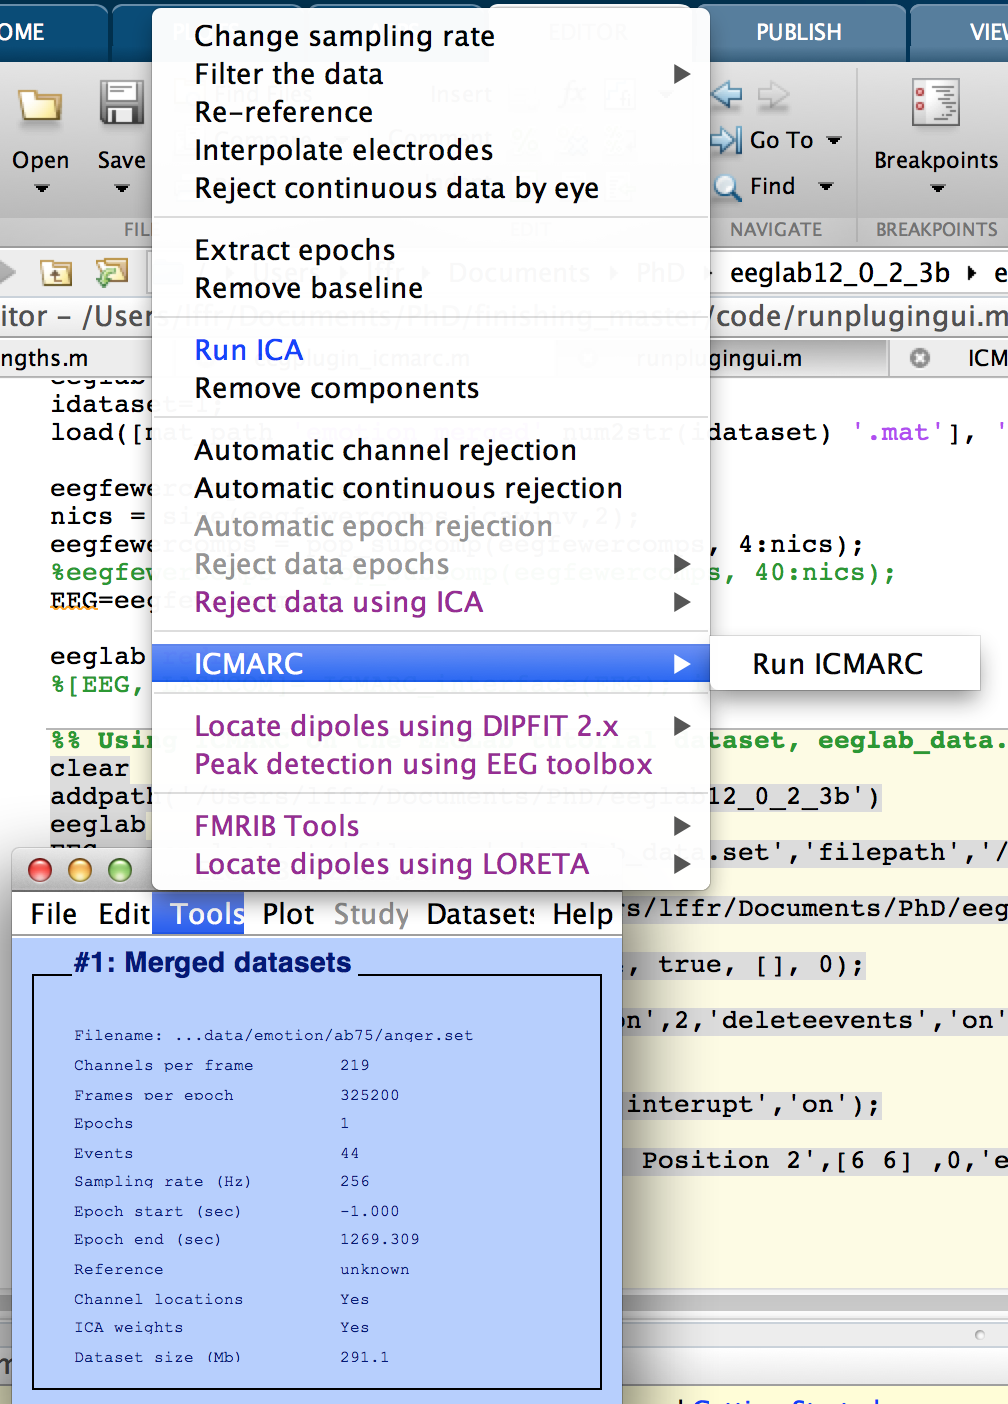
\includegraphics[width=0.5\textwidth]{figs/runICMARC}
\caption{The submenu that starts the classification of ICs using IC\_MARC.}
\label{fig:runICMARC}
\end{figure}

The first input to \textit{pop\_ICMARC\_interface} is which feature
set to use. There are three possibilities:
``established\_spatial\_features'', ``spatial2'', and
``established\_features''. These are the three feature sets for which
classifiers have been trained. The feature set
``established\_spatial\_features'' consists solely of spatial features
and seems to perform the best over most datasets (based on
undocumented experience). This is also the default which will be used
if the user does not change the feature set value in the window. The
feature set ``spatial2'' also consists of only spatial features, but
has no features derived from the dipole fit, which may take a long
time to obtain. It was optimised manually to obtain a compromise
between speed of feature calculation and classification
performance. The final feature set, ``established\_features'', was
optimised automatically within one study as described
in~\cite{fro14}. This contains both spatial, temporal, and spectral
features.

The second input to \textit{pop\_ICMARC\_interface} determines whether
or not to perform pre-processing steps for temporal and spectral
features if no spectral or temporal features are included in the
requested feature set. This is a checkbox that, if set, forces the
pre-processing steps to be performed. If unchecked (the default),
pre-processing steps for temporal and spectral features are skipped if
no such features are included in the requested feature set to save time.

\begin{figure}
\center
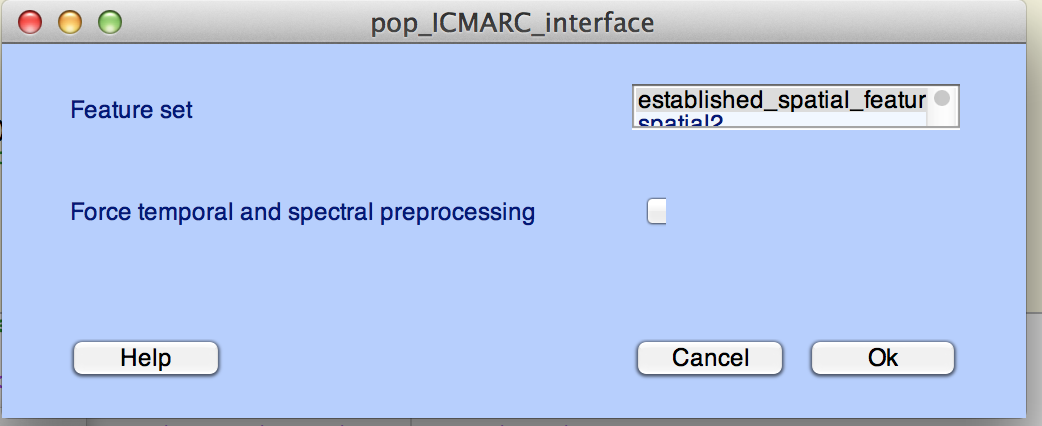
\includegraphics[width=0.8\textwidth]{figs/pop_ICMARC_interface}
\caption{The pop up window for starting IC\_MARC.}
\label{fig:popICMARCinterface}
\end{figure}


\subsection{Plot classified ICs (Plot menu)}
Upon clicking ``Plot scalpmaps with classes'' in the ``ICMARC''
submenu of the Plot menu, the scalpmaps of all ICs in the EEG data
structure are plotted below buttons labeled with their respective
classes as shown in Figure~\ref{fig:scalpmapsAndClasses}. 

\begin{figure}
\center
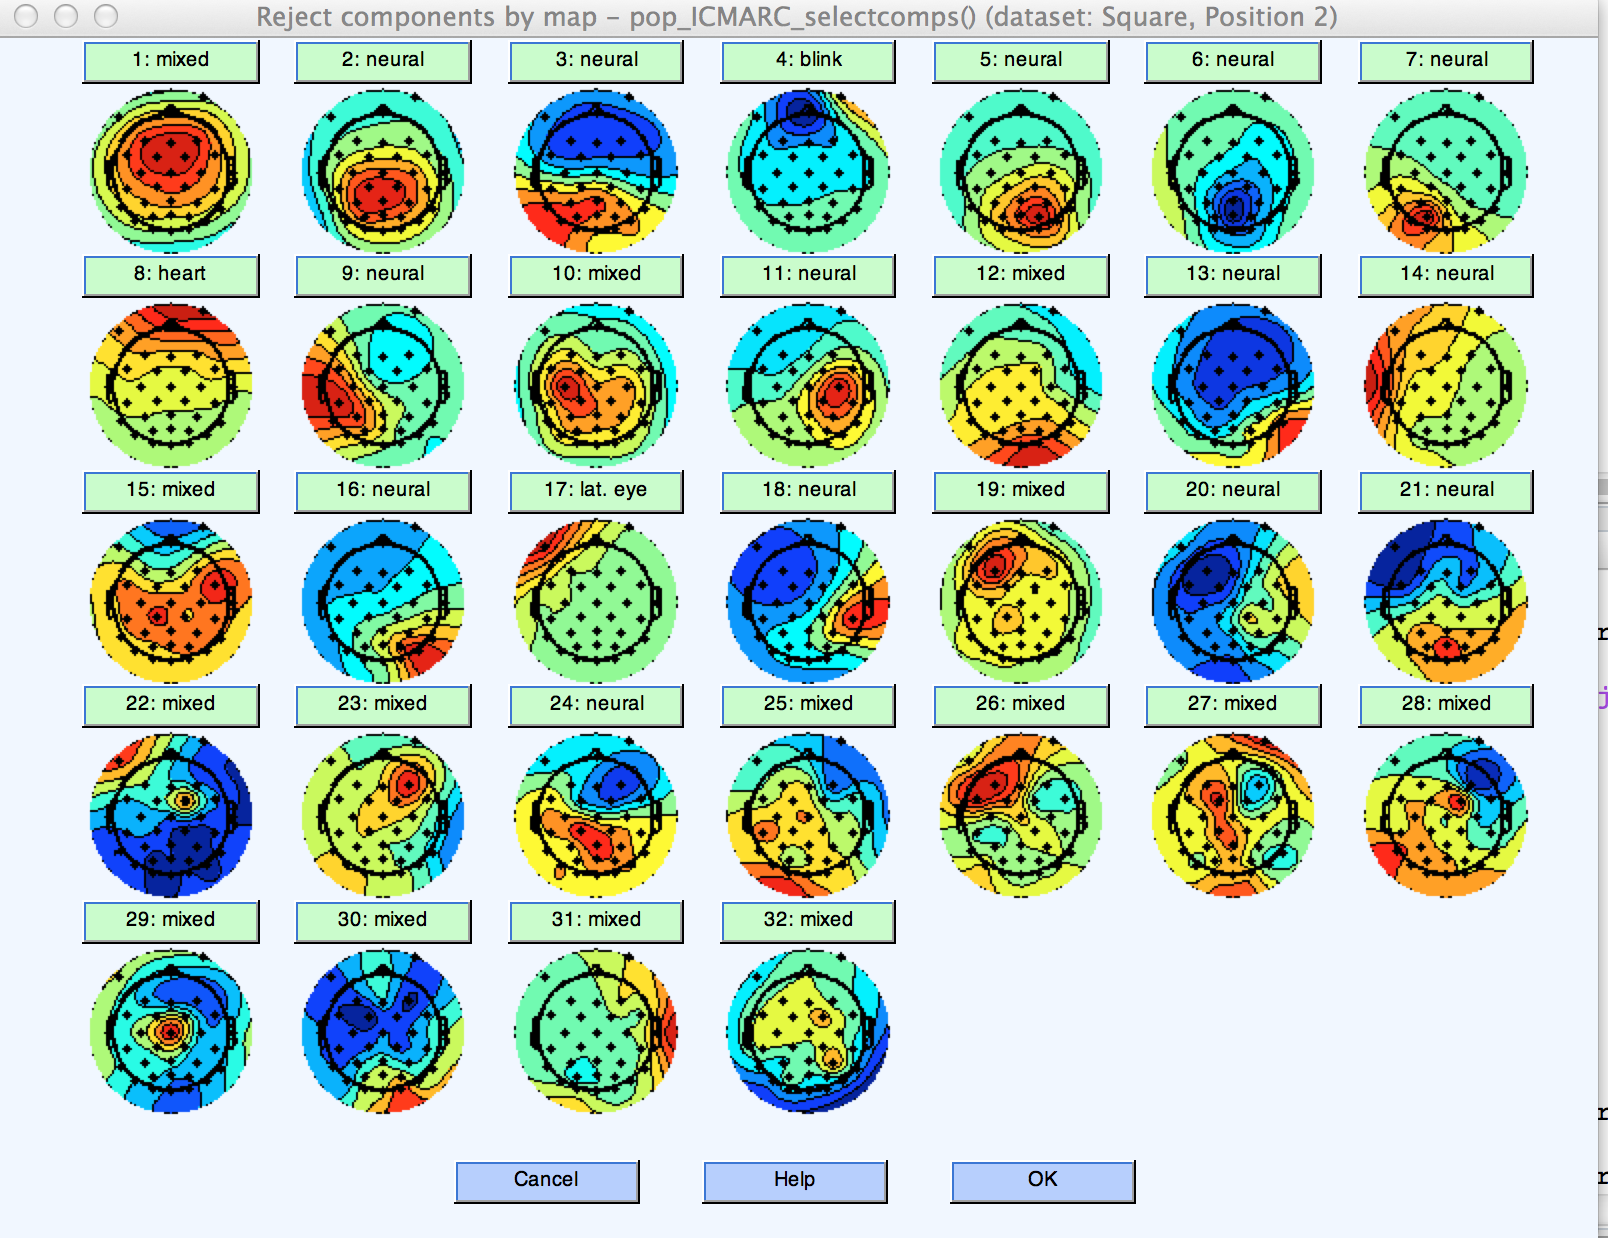
\includegraphics[width=0.8\textwidth]{figs/scalpmaps_and_classes}
\caption{Plot of scalpmaps and their predicted classes.}
\label{fig:scalpmapsAndClasses}
\end{figure}

The buttons labeled with the IC classes can be clicked to inspect the
power spectrum and, if epochs are present in the EEG data
set, an ERP image for each IC in a window such as that shown in
Figure~\ref{fig:changeClass}. This window also allows the user to
change the class of the IC. The ERP image will be empty if epochs are
not present.

In the case of many ICs in the EEG data set, several windows
containing ICs and their labels will pop up. If the cancel button of
such a window is clicked, only the changes made in that window will be
canceled while the changes made to the ICs contained in the other windows
will be retained if the OK buttons of those windows are clicked.

\begin{figure}
\center
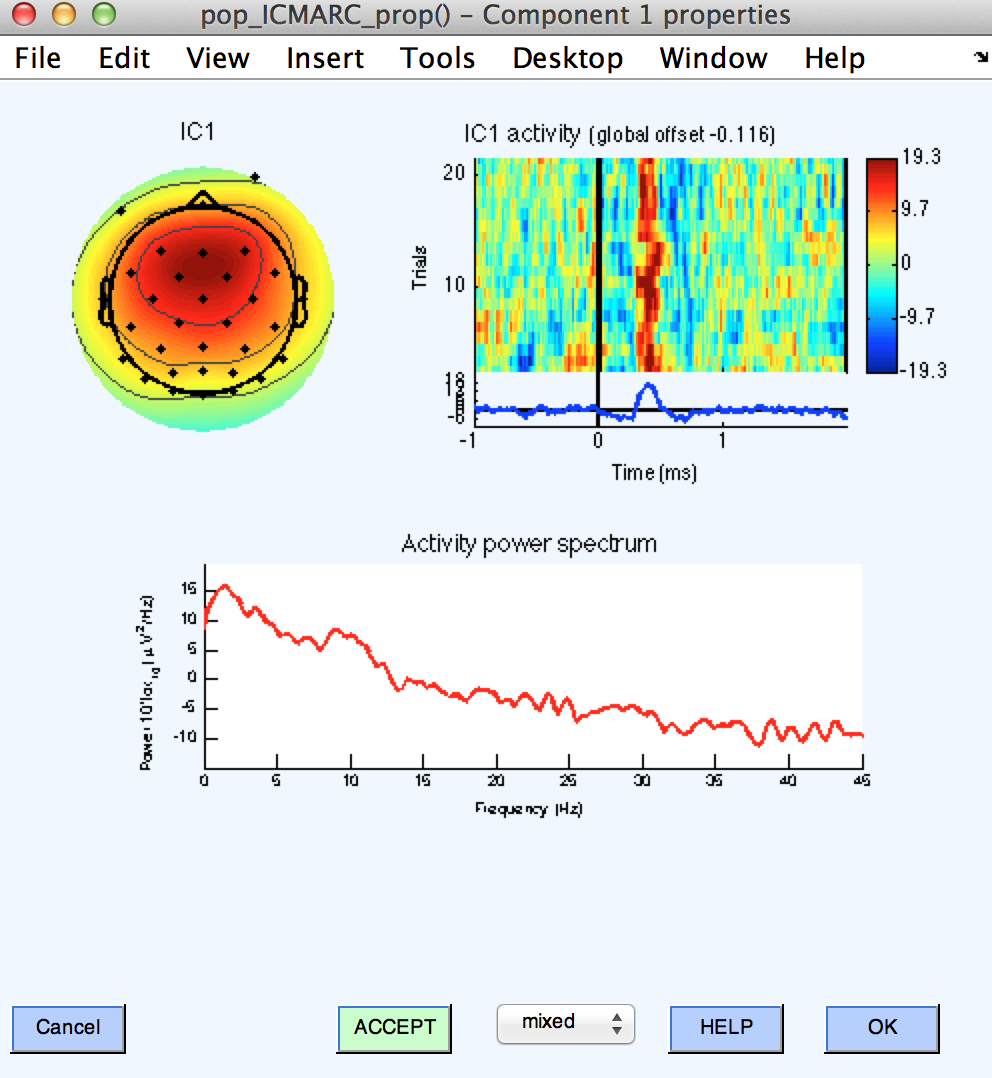
\includegraphics[width=0.8\textwidth]{figs/changeClass}
\caption{Inspect power spectrum, ERP image and change class of IC.}
\label{fig:changeClass}
\end{figure}

If the field EEG.reject.classtype is empty or not present, the classes
of all ICs are initialized as type ``mixed'' and a window pops up to
warn of this as shown in Figure~\ref{fig:noclasseswarning}. This
allows the user to manually classify ICs while making sure that the
manual classifications are stored in the field
EEG.reject.classtype. The dropdown menu for manual classifications
also contains a ``loose electrode'' class.

\begin{figure}
\center
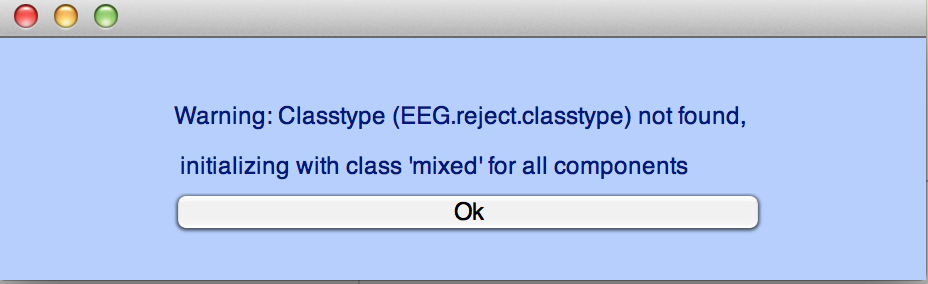
\includegraphics[width=0.8\textwidth]{figs/noclasseswarning}
\caption{The warning that pops up if the field EEG.reject.classtype is
  empty or not present when ``Plot scalpmaps with classes'' in the
  Plot menu is clicked.}
\label{fig:noclasseswarning}
\end{figure}

\section{Bugs and request}
If you run into problems using this plug-in, please send an e-mail to
laura.frolich@gmail.com and I will do my best to help. Also, if you
would like to assist in improving the classifier I would be very
grateful for access to EEG data sets containing manually labeled ICs
to use as training data to explore further improvements.

\clearpage

\bibliography{refs}{}
\bibliographystyle{plain}

\end{document}
